\chapter{DebugWire}
\section{Descrizione del protocollo e fondamentali}

Parte fondamentale del core AVR, omessa dal diagramma in figura~\ref{fig:avr-arch}, è il sistema di \textit{debugging} on chip ``\textit{DebugWire}''.

Esso permette, tramite un tool esterno collegato all'integrato, di stallare la cpu e leggere e scrivere le memorie e i registri.\cite[sec 25]{avr:m328p}

Affinché le funzionalità di debugging siano disponibili, è necessario abilitare la periferica DebugWire tramite i bit di configurazione al momento della programmazione del dispositivo\cite[tab 28-7]{avr:m328p}.

\subsection{Interfaccia fisica}\label{ss:dw-phy}

L'interfacciamento fisico tra controllore e dispositivo esterno avviene tramite una sola connessione al pin di reset dell'integrato \textit{target}.

Il fatto che l'interfaccia di debug sia collocata sul pin di reset comporta che, una volta abilitata la periferica DebugWire, non sia più possibile resettare il dispositivo o programmarlo tramite interfaccia ISP\cites{avr:appnote:isp}[sec 25.3]{avr:m328p}, ma si rende necessaria una procedura di disattivazione temporanea o la possibilità di programmare l'integrato tramite il protocollo DebugWire.

La comunicazione tra programmatore e target è di tipo seriale e half duplex data la natura della connessione. In particolare il protocollo utilizzato è una derivazione di una seriale UART su un bus open collector, come è osservabile dalla figura~\ref{fig:dw-schematic}\cite{site:dw-reverse-engeneering}.

\begin{figure}[t]
    \centering
    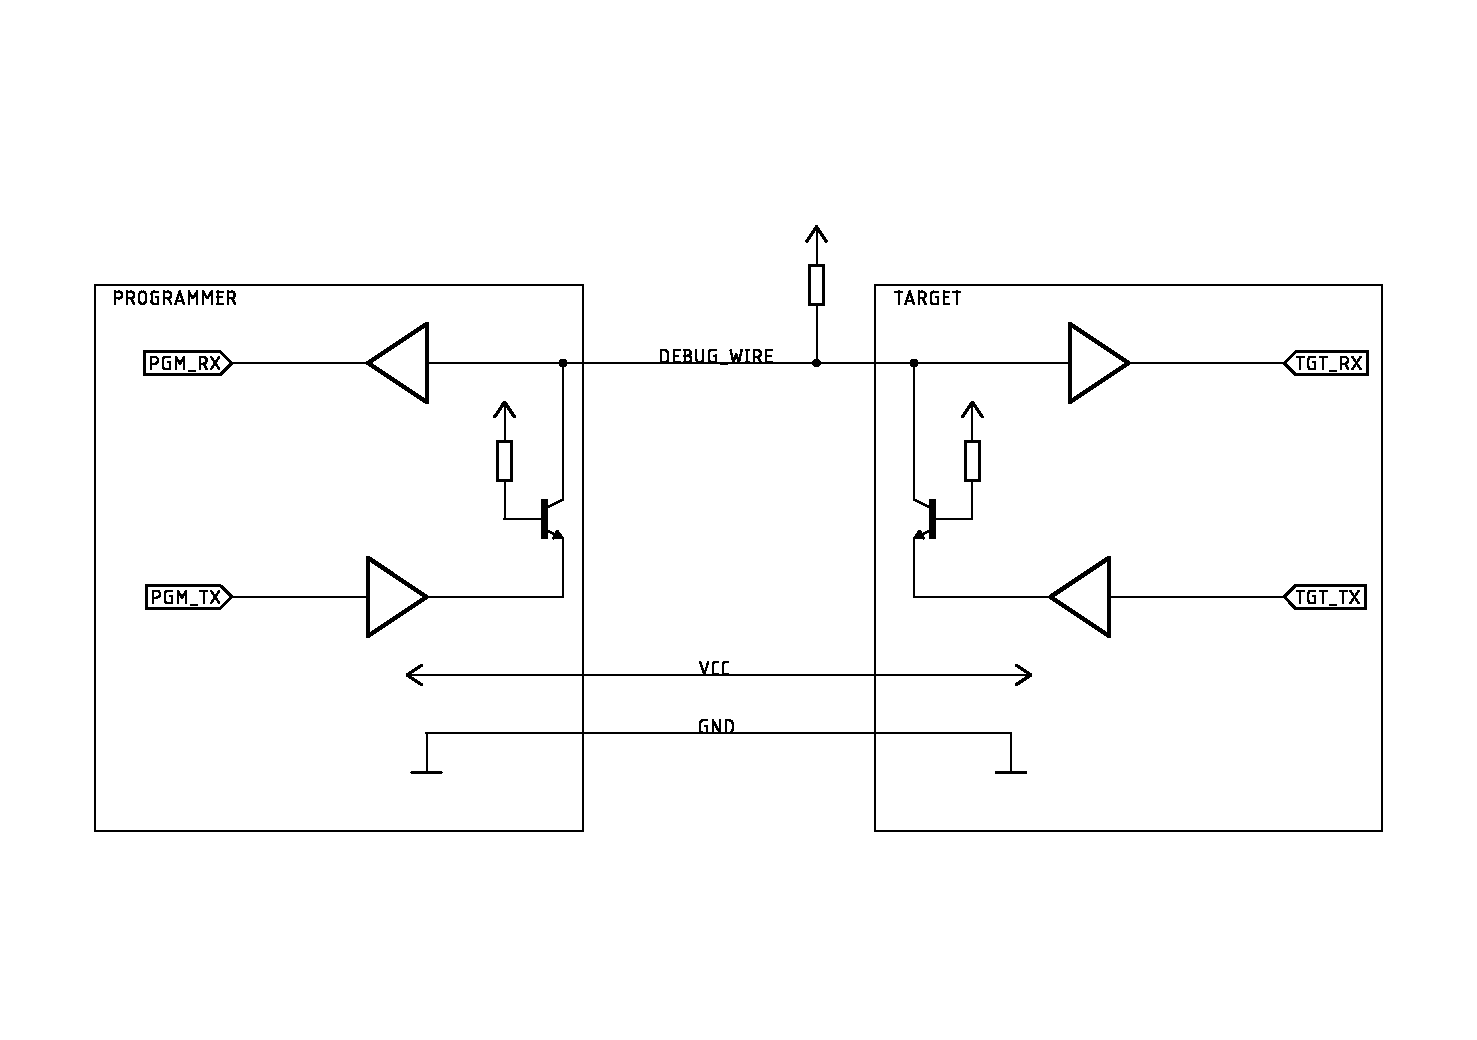
\includegraphics[width=\textwidth]{dw-schematic.pdf}
    \caption[]{Schema concettuale del funzionamento dell'interconnessione tra programmatore e controllore target per il protocollo DebugWire}\label{fig:dw-schematic}
\end{figure}

\subsubsection{Protocollo UART}\label{ss:uart}

Il protocollo UART è un metodo di trasmissione punto-punto digitale seriale asincrono che generalmente lavora su due connessioni tra i due attori della comunicazione. Le due linee rimangono a livello logico 1 quando non c'è attività.

Le linee prendono il nome di ``TX'' e ``RX'' in funzione dell'utilizzo che la periferica master ne fa: è necessario notare come le due linee vengano ``incrociate'' in modo tale da far sì che il pin di trasmissione di un attore vada a collegarsi con il pin di ricezione della controparte.

Essendo un protocollo asincrono, ovvero vi è assenza di una linea di sincronizzazione (clock), le due parti della comunicazione devono conoscere a priori la velocità e il formato dei dati attesi sulle linee.

La trasmissione inizia con un periodo di livello logico 0 (\textit{Start Bit}), in modo che sia possibile l'identificazione dell'inizio della trasmissione di un simbolo rilevando il fronte di transizione da livello logico 1 a livello logico 0 (\textit{Falling Edge}).

Durante questo tempo di bit dove la linea di trasmissione è a livello logico 0 è dunque possibile inizializzare l'hardware e sincronizzare le sorgenti di clock per la ricezione. In seguito al bit di inizio si susseguono i bit del dato, dal meno significativo al più significativo, con periodo pari al tempo di bit stesso. In funzione della specifica del protocollo possono essere inviate unità di dati fondamentali di dimensione da 5 a 8 bit.

A seguito dei bit di dati viene quindi inviato opzionalmente un bit di parità per garantire l'integrità dei dati e successivamente la linea viene posta a livello logico 1 per uno o due periodi di bit, permettendo al ricevitore di eseguire operazioni e resettare la macchina a stati per la ricezione dell'eventuale simbolo seguente.\cite{site:rs-uart}

Essendo un sistema asincrono è opportuno ipotizzare il disallineamento delle frequenze di invio e campionamento: in tal caso una desincronizzazione può essere tollerata se entro il limite dato dall'equazione~\ref{eq:uart-max-delay}
\begin{equation}\label{eq:uart-max-delay}
    t_{delay_{\max}} = \frac{1}{2}(N_{data}+N_{parity}+N_{stop}+1)t_{bit}    
\end{equation}
dove \(N_{data}\) è il numero di bit contenuti nel simbolo inviato che è stato negoziato, \(N_{parity}\) indica il numero di bit di parità, \(N_{stop}\) il numero di \textit{stop bits} e \(t_{bit}\) è il tempo per bit. Inoltre si tiene conto del bit di inizio (\textit{start bit}). Questo comportamento può essere notato dalla figura~\ref{fig:uart-sync}, dove vengono rappresentati il caso ideale e il caso di desincronizzazione massima. In ogni caso si ha che il campionamento avviene all'interno del bit in invio.

\afterpage{
    \begin{figure}[ht]
        \centering
        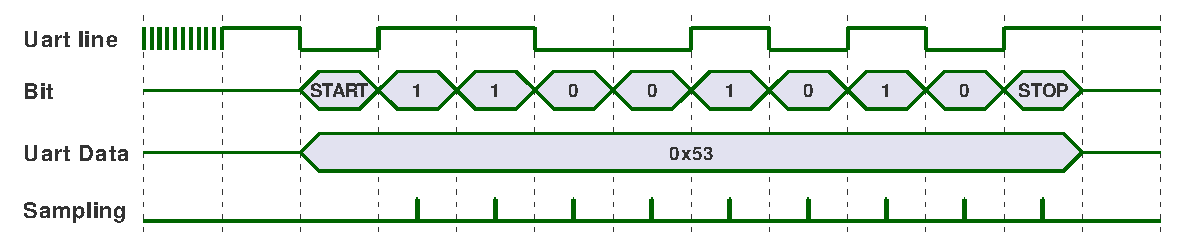
\includegraphics[width=.8\textwidth]{uart-timings.pdf}\\
        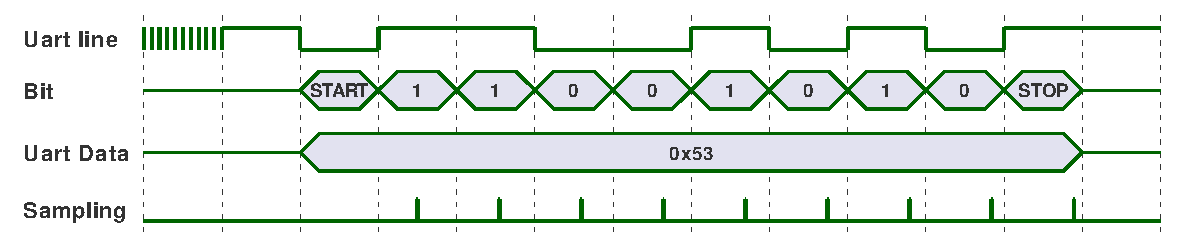
\includegraphics[width=.8\textwidth]{uart-timings-unsync.pdf}
        \caption[]{I diagrammi di sequenza dimostrano che, anche in caso di non sincronizzazione delle frequenze di invio e ricezione viene mantenuta l'integrità dei dati trasmessi. Viene mostrata una comunicazione seriale 8N1\footnote{Definizione della configurazione di una linea seriale. Essa è composta da tre caratteri: <Numero di bit dati><Tipo di parità ([N]one, [O]dd, [E]ven, [M]ark, [S]pace)><Numero di Stop bits>}}\label{fig:uart-sync}
    \end{figure}
}

La motivazione per cui il campionamento avviene a metà del tempo di bit è data dal fatto che la desincronizzazione può essere causata da una frequenza più alta o più bassa, per cui vale la relazione descritta dall'equazione~\ref{eq:uart-period-receive-delay}
\begin{equation}\label{eq:uart-period-receive-delay}
     t_{bit_{recv}} = t_{bit_{snd}} \pm t_{delay_{\max}}
\end{equation}

Infine, se la velocità di trasmissione fosse misurata in \textit{bit per secondo}, secondo la formula \(v_{uart} = \frac{1}{t_{bit}}\), essa non sarebbe veritiera e porterebbe confusione, in quanto la formula sopra enunciata includa nel conteggio dei bit trasmessi anche i bit di controllo (Start, parity e Stop bit) i quali non contribuiscono all'informazione inviata. Di conseguenza è opportuno definire la velocità di trasmissione della linea seriale come il numero di simboli trasmessi per secondo. Questa definizione differisce dalla prima un quanto il simbolo è composto da un numero di bit non necessariamente pari a 8.

È possibile determinare la velocità in baud a partire dal bitrate e dalla configurazione della linea UART secondo la relazione~\ref{eq:baud-from-bit-rate}\cite{site:baud}:
\begin{equation}\label{eq:baud-from-bit-rate}
    v_{tx_{baud}} = \frac{1}{t_{bit}(N_{data} + N_{parity} + N_{stop} + 1)}
\end{equation}

Da quanto è possibile dedurre dall'equazione~\ref{eq:baud-from-bit-rate}, l'effettivo bit rate di trasmissione della linea UART differisca di un fattore di \(\frac{N_{data}}{N_{data} + N_{parity} + N_{stop} + 1}\) rispetto al bitrate grezzo di trasmissione \(v_{uart}\)

\subsection{Funzionamento}

Tutte le comunicazioni che avvengono sul bus DebugWire non hanno alcun tipo di verifica dell'integrità del dato (Serial 8N1). La comunicazione può avvenire in qualsiasi momento.

In particolare il reset della comunicazione tra target e programmatore/debugger avviene mediante l'invio di un BREAK\footnote{La linea viene posta a livello logico 0 per più di 9 tempi di bit} sulla linea.
Ogni qualvolta sia rilevato un errore (per esempio viene ricevuto un byte inatteso o un comando non noto), il primo attore che rileva l'errore invierà un BREAK che causerà il reset della controparte.

Ciò è possibile perché la connessione è un bus open collector: il conflitto di accesso avviene solo ponendo la linea a livello logico 0 e non comporta cortocircuitazioni di qualsiasi genere. Il conflitto viene rilevato quando un attore legge dal bus uno stato diverso da quanto inviato durante la trasmissione del bit (in particolare quando l'attore riceve un bit pari a 0 quando sta inviando un bit di valore 1).

La velocità di comunicazione è invece definita in funzione della frequenza della cpu del target. Nell'hardware della periferica è presente un \textit{prescaler} (il cui valore di default è di 128) e la velocità di comunicazione viene stabilita come \[v_{com} = \frac{f_{cpu} [Hz]}{prescaler}[bps]\]

Ad ogni reset della comunicazione il prescaler viene resettato al valore iniziale.

In risposta ad un BREAK il target risponderà sempre con l'invio di un valore noto (0x55), facendo sì che a livello fisico sia inviata un'onda quadra con frequenza \(v_{com}\)\cite{site:dw-reverse-engeneering} (si veda figura~\ref{fig:dw-timings})

\begin{figure}[ht]
    \centering
    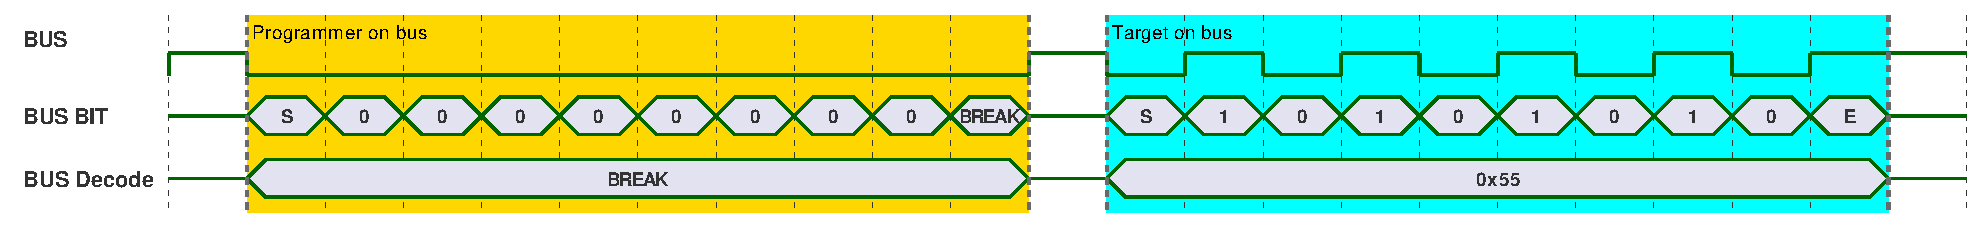
\includegraphics[width=\textwidth]{dw-break.pdf}
    \caption[]{Diagramma delle tempistiche del bus DebugWire durante il reset della trasmissione}\label{fig:dw-timings}
\end{figure}

È dunque possibile definire un algoritmo per l'inizializzazione della sessione in modo che la frequenza della trasmissione venga dedotta dalla risposta del target invece che essere nota a priori, permettendo un untilizzo semplificato della periferica.

L'algoritmo è strutturato come segue
\begin{enumerate}
    \item Preparazione dell'hardware e inizializzazione strutture dati
    \item Invio di un break dalla durata di 100ms. La durata viene stabilita in funzione della frequenza di trasmissione ragionevolmente più bassa possibile: Considerando che la famiglia AVR integra nei suoi controllori un oscillatore RC a 128kHz usato comunemente per operazioni ``low power'' e ipotizzando che sia abilitata la funzionalità di divisione del clock per un fattore di 8\cite[sec 9.11, tab 28-9]{avr:m328p}, si ottiene una frequenza del core di 16kHz. Ponendo quindi il prescaler di comunicazione DebugWire a 128 otteniamo una frequenza di trasmissione di 125Hz, ovvero 8ms per bit. Infine, sapendo che il tempo di break consiste in almeno 10 bit trasmessi a 0, si ottiene un tempo minimo di break di 80ms, arrotondato a 100ms
    \item Attesa del primo fronte di transizione da livello logico 1 a livello logico 0
    \item Attesa del successivo fronte di transizione da livello logico 0 a livello logico 1 (calcolando il tempo intercorso tra i due fronti)
\end{enumerate}

A questo punto è possibile trovare la frequenza di bit dalla quale ricavare il baud rate.

\subsection{Comandi e features}

Una volta che la cpu del controllore target è in stato \textit{halt} è possibile interagire con la periferica DebugWire per eseguire le operazioni di debug. A seguito di un BREAK e successiva risposta è possibile interpellare il controllore con i comandi descritti di seguito.

Vi sono due classi di comandi: comandi basilari e comandi composti.
I primi sono comandi che svolgono azioni semplici e definite staticamente, quali la scrittura del Program Counter, Instruction register, scrittura del registro di breakpoint hardware e configurazione di flag e comunicazione. Tramite questi comandi è possibile definire i limiti di scrittura/lettura delle memorie e eseguire istruzioni.
I Secondi sono operazioni complesse che necessitano parametri di configurazione i quali sono impostati tramite comandi basilari.

I comandi disponibili per l'interazione con il microcontrollore target tramite DebugWire sono limitati e appartengono a quattro categorie: \textit{Communication Settings}, \textit{Flag Setting},\textit{Program Flow Control} e \textit{Memory R/W}.

\subsubsection{Communication Settings}

Questi comandi vengono utilizzati per modificare il valore del prescaler di comunicazione in modo da variare la velocità di trasmissione. Sono comandi particolarmente utili nel debugging di controllori a bassa frequenza (128kHz).

Non vi è una logica nota nell'assegnazione del comando al corrispondente valore del prescaler: si rende necessaria una tabella di associazione come riportato dalla tabella~\ref{tab:dw-presc-settings}

\begin{table}[ht]
    \centering
    \begin{tabular}{ c c c }
        \textbf{Comando} & \textbf{Valore del prescaler} & \textbf{Bitrate a 16MHz} \\
        \hline
        0x83 & 128 & 125kbps \\
        0x82 & 64 & 254kbps \\
        0x81 & 32 & 500kbps \\
        0x80 & 16 & 1Mbps \\
        0xA0 & 8 & 2Mbps \\
        0xA1 & 4 & 4Mbps \\
        0xA2 & 2 & 8Mbps \\
        0xA3 & 1 & 16Mbps \\
        \hline
    \end{tabular}
    \caption[]{Tabella descrittiva dei comandi per la modifica del prescaler di trasmissione della periferica di debug del controllore target\cite{site:dw-reverse-engeneering}}\label{tab:dw-presc-settings}
\end{table}

Una volta inviato il comando di configurazione del prescaler il controllore si adatterà alla velocità richiesta e risponderà con il valore \texttt{0x55} inviato alla nuova frequenza. Questo valore può essere usato per settare adattivamente la frequenza del programmatore oppure per verificare che le impostazioni siano corrette.

\subsubsection{Flag Setting}

È necessario configurare lo stato della periferica prima di eseguire effettivamente le operazioni che sono state preparate. Possiamo chiamare questo stato ``Contesto di esecuzione'' in quanto la stessa configurazione dell'hardware permette di eseguire diverse azioni in funzione del contesto che viene configurato.

I contesti disponibili sono elencati nella tabella~\ref{tab:dw-contexts}.

\begin{table}[ht]
    \centering
    \begin{tabular}{ c l }
        \textbf{Comando dW} & \textbf{Contesto} \\
        \hline
        0x60 & Ripresa dell'esecuzione\\
        0x61 & Ripresa dell'esecuzione fino all'indirizzo HWBP\\
        0x64 & Lettura/Scrittura memoria Flash\\
        0x66 & Lettura/Scrittura della SRAM\\
        0x79 & Riprese dell'esecuzione usando l'istruzione caricata\\
        0x7A & Single Step\\
        \hline
    \end{tabular}
    \caption[]{Tabella descrittiva dei contesti di esecuzione DebugWire\cite{site:dw-reverse-engeneering}}\label{tab:dw-contexts}
\end{table}

È possibile inoltre modificare i contesti ponendo il valore del bit 5 a zero per permettere alle periferiche di temporizzazione (timers) di continuare il conteggio durante lo stepping.

\subsubsection{Program Flow Control}

Questi comandi sono utilizzati per confermare le operazioni da eseguire.

Esistono comandi di ``GO'' per le varie operazioni composite quali la lettura e scrittura della memoria SRAM (0x20 per indirizzi multipli, 0x21 per un indirizzo singolo), esecuzione di un'istruzione precedentemente caricata in IR senza incrementare il program counter (0x23), ripresa dell'esecuzione (0x30) o single stepping (0x31).

Se il bit 5 è settato allora il target effettuerà il reset della sessione inviando un BREAK seguito da 0x55 al termine dell'esecuzione.

\subsubsection{Memory R/W}

Questi sono i comandi fondamentali per la scrittura e lettura dei registri PC, IR, HWBP e SIGNATURE (sola lettura).

Questi registri possono essere trattati opportunamente a seconda della loro funzione oppure possono essere visti come parametri di configurazione per le operazioni composite descritte in seguito.

I registri di configurazione sono mappati da un indice come descritto dalla tabella\ref{tab:dw-regs-idx}.

\begin{table}[ht]
    \centering
    \begin{tabular}{ c l }
        \textbf{Indice} & \textbf{Registro associato} \\
        \hline
        0 & Program Counter (PC)\\
        1 & Hardware Breakpoint (HWBP)\\
        2 & Instruction Register IR\\
        3 & DW Signature register\\
        \hline
    \end{tabular}
    \caption[]{Tabella descrittiva dell'associazione degli indici ai registri elementari\cite{site:dw-reverse-engeneering}}\label{tab:dw-regs-idx}
\end{table}

Le operazioni di lettura e scrittura dei registri avvengono mediante l'invio di pacchetti come definito dalle figure~\ref{fig:dw-reg-wrt}~e~\ref{fig:dw-reg-rd}

\begin{figure}[ht]

    \centering
    \begin{bytefield}[endianness=big,bitwidth=1em]{24}
        \bitheader{0-23}\\
        \bitbox{4}{0xD} & \bitbox{4}{idx} & \bitbox{16}{data}\\
    \end{bytefield}

    \caption[]{Pacchetto di scrittura di un registro elementare. Nessuna risposta da parte del target}\label{fig:dw-reg-wrt}
\end{figure}


\begin{figure}[ht]

    \centering

    \begin{lrbox}{\bytefieldbox}
        \begin{bytefield}[endianness=big,bitwidth=1em]{8}
            \bitheader{0-7}\\
            \bitbox{4}{0xF} & \bitbox{4}{idx} \\
        \end{bytefield}
    \end{lrbox}
    \subfloat[]{\usebox{\bytefieldbox}}

    \vspace*{5mm}%
    \begin{lrbox}{\bytefieldbox}
        \begin{bytefield}[endianness=big,bitwidth=1em]{16}
            \bitheader{0-15}\\
            \bitbox{16}{data}\\
        \end{bytefield}
    \end{lrbox}
    \subfloat[]{\usebox{\bytefieldbox}}


    \caption[]{Pacchetto di lettura di un registro elementare (a) e successiva risposta (b)}\label{fig:dw-reg-rd}
\end{figure}

\subsubsection{Comandi compositi}

DebugWire permette di leggere e scrivere la memoria SRAM mediante una combinazione di comandi elementari.
Grazie a questa funzionalità è possibile leggere e scrivere sia la memoria dati che i registri di configurazione delle periferiche e i registri ``general purpose'' come viene evidenziato dalla figura~\ref{fig:avr-sram-alloc}.

L'algoritmo per la scrittura dei registri (r0-r31) consiste in quanto segue\cite{site:dw-reverse-engeneering}:
\begin{enumerate}
    \item Context: SRAM R/W
    \item Scrittura del registro iniziale nel registro PC
    \item Scrittura del registro finale nel registro HWBP
    \item Selezione modalità (Comando C2 seguito dall'indice dell'operazione come descritto nella tabella~\ref{tab:dw-ops})
    \item GO SRAM R/W
    \item (Se scrittura) Invio dei byte da scrivere.\\(Se lettura) Ricezione dei byte letti.
\end{enumerate}

\begin{table}[t]
    \centering
    \begin{tabular}{ c l }
        \textbf{Indice} & \textbf{Modalità} \\
        \hline
        0 & Lettura memoria SRAM\\
        1 & Lettura registri \\
        2 & Lettura memoria Flash\\
        4 & Scrittura memoria SRAM\\
        5 & Scrittura registri\\
        \hline
    \end{tabular}
    \caption[]{Tabella descrittiva dell'associazione degli indici alle modalità di operazione sulle memorie\cite{site:dw-reverse-engeneering}}\label{tab:dw-ops}
\end{table}

Di seguito, alla figura~\ref{fig:dw-reg-rw-com}, viene riportata la traccia di comunicazione per questo algoritmo.

Analogamente è possibile leggere e scrivere la memoria SRAM e leggere la memoria FLASH con il seguente algoritmo:
\begin{enumerate}
    \item Scrittura dell'indirizzo di partenza nella coppia di registri \texttt{r30 - r31}
    \item Scrittura del registro PC al valore 0x0000 se lettura o 0x0001 se scrittura
    \item Scrittura del doppio della lunghezza dei dati (+1 se in scrittura) da leggere/scrivere registro HWBP
    \item Selezione modalità
    \item GO con appropriata modalità.
\end{enumerate}

\begin{figure}[p]

    \centering
    \begin{bytefield}[endianness=big,bitwidth=1em]{32}
        \bitheader{0-31}\\
        \bitbox{8}{CNTX\_SRAM} & \bitbox{8}{0xD0} & \bitbox{16}{start\_reg} \\
        \bitbox{8}{0xD1} & \bitbox{16}{end\_reg + 1} & \bitbox{8}{0xC2} \\
        \bitbox{8}{MOD: 0x00/0x05} & \bitbox{8}{GO MEM}
    \end{bytefield}

    \caption[]{Comunicazione inviata dal debugger per leggere/scrivere i registri. In caso di scrittura viene seguita da (end\_reg - start\_reg) byte, altrimenti la stessa quantità di byte viene ricevuta.}\label{fig:dw-reg-rw-com}
\end{figure}

\begin{figure}[p]

    \centering
    \begin{bytefield}[endianness=big,bitwidth=1em]{32}
        \bitheader{0-31}\\
        \bitbox{8}{CNTX\_SRAM} & \bitbox{24}{0xD0001E} \\
        \bitbox{24}{0xD10020} & \bitbox{8}{0xC2} \\
        \bitbox{8}{0x05} & \bitbox{8}{0x20} & \bitbox{16}{addr\_start} \\
        \bitbox{8}{0xC2} & \bitbox{8}{0x04/0x00/0x01} & \bitbox{16}{0xD000} \\
        \bitbox{8}{0x00/0x01} & \bitbox{8}{0xD1} & \bitbox{16}{len * 2 (+1 if wrt)}\\
        \bitbox{8}{GO MEM}
    \end{bytefield}

    \caption[]{Comunicazione inviata dal debugger per leggere/scrivere le memorie. In caso di scrittura viene seguita da \textit{len} byte, altrimenti la stessa quantità di byte viene ricevuta.}\label{fig:dw-mem-rw-com}
\end{figure}

Alla figura~\ref{fig:dw-mem-rw-com}, viene riportata la traccia di comunicazione per questo algoritmo.

È possibile eseguire direttamente un'istruzione senza scriverla nella memoria Flash. In questo caso è sufficiente scrivere nel registro IR l'opcode dell'operazione ed eseguire il comando di flow control (0x23 o 0x33). Si noti che non è possibile eseguire istruzioni di 32 bit.

Si noti come i valori dei registri \texttt{Z, PC, HWBP e IR} vengano modificati da queste operazioni. Ciò rende necessaria una procedura di salvataggio e ripristino prima di riprendere l'eventuale esecuzione del codice sul dispositivo \textit{target}.

\section{Funzionalità aggiuntive}

Grazie alla possibilità di eseguire istruzioni arbitrarie tramite l'interfaccia di debug, è possibile creare delle funzionalità non previste dal protocollo stesso ma di notevole importanza per la gestione del debug.

\subsection{Riconoscimento del target}

Durante l'inizializzazione il debugger leggerà il registro SIGNATURE DebugWire per identificare il componente.

Una sezione di memoria flash è stata dedicata al salvataggio di una struttura dati contenente le informazioni necessarie al debugging di un integrato, per cui è sufficiente cercare sequenzialmente la coincidenza del valore del registro signature rispetto al campo id.

La struttura salvata contenente gli indirizzi e le dimensioni viene mostrata con il listato~\ref{lst:struct-dw-dev}

\noindent\begin{minipage}{\textwidth}
    \begin{lstlisting}[style=C, caption={Strutture utilizzate nel codice finale per il salvataggio e la ricerca dei parametri associati al target connesso}, label=lst:struct-dw-dev]
    typedef struct dw_device_definition{
        uint16_t signature;

        uint16_t sram_base;         //first sram address after extended io
        uint16_t sram_end;          //first sram address after extended io

        uint8_t flash_page_end;     //words per page
        uint16_t flash_end;         //last flash valid word

        uint16_t eeprom_end;        //first eeporom address after io and extended io

        uint8_t reg_spmcsr;
        uint8_t reg_dwdr;
        uint8_t reg_eearl;
        uint8_t reg_eecr;
        uint8_t reg_eedr;
    } __attribute__((packed)) dw_device_definition_t;

    struct dw_devices{
        uint16_t items;
        dw_device_definition_t devices[];
    } __attribute__((packed));
    \end{lstlisting}
\end{minipage}

\subsection{Programmazione delle memorie non volatili}

In particolare il protocollo DebugWire non permette di accedere in scrittura alle memorie non volatili, impedendone così la programmazione tramite tale interfaccia.

Prendendo spunto da quanto riportato sul datasheet della maggior parte dei dispositivi AVR\cite[34]{avr:m328p}\cite[sec 26.2.5]{avr:m328p}, è possibile ideare una breve routine eseguibile passo-passo dal debugger per la scrittura di tali memorie.

Bisogna però trovare un modo per inviare il dato, o i dati, da scrivere nella memoria.

Una possibile soluzione potrebbe essere quella di scrivere il byte o la pagina in RAM e utilizzare così istruzioni \texttt{ld}, ma questo approccio richiederebbe troppe istruzioni e causerebbe lunghi tempi di programmazione.

La soluzione adottata è quella di leggere o scrivere il registro \texttt{DWDR}. Dati i test eseguiti, una scrittura del registro tramite i comandi sopra descritti (il registro si trova ad un indirizzo noto) richiede un ulteriore byte inviato sulla linea seriale che verrà salvato in tale registro\cite{site:dw-reverse-engeneering}. Analogamente la sua lettura comporta un ulteriore byte inviato dal target rappresentate il valore salvato\cite{site:dw-reverse-engeneering}.

Sono stati elaborati due frammenti di codice eseguibili dal debugger per la programmazione delle memorie non volati. Essi sono consultabili nell'appendice come documento~\ref{app:dw-flash-prog} e documento~\ref{app:dw-eeprom-prog}.

Da tali documenti possiamo osservare come il codice sia fortemente dipendente dal debugger per la preparazione del contesto, ovvero necessita che prima dell'esecuzione siano eseguite certe istruzioni di preparazione quali salvataggio dello stato dei registri e preparazione delle costanti e indirizzi nei registri utilizzati.

Inoltre la scrittura dell'algoritmo di programmazione della memoria flash è stata fatta facendo sì che non sia necessario istanziare un buffer contenente l'intera pagina da programmare precedentemente alla chiamata, bensì è possibile scrivere il buffer temporaneo a blocchi di dimensione indefinita purché venga completato prima di procedere.

Questo permette di scrivere codice a bassissimo impatto sulla quantità di memoria SRAM utilizzata per buffer temporanei, condizione necessaria per lo sviluppo su ATMega16U2 in quanto la memoria SRAM totale disponibile non supera i 512byte\cite{avr:m16u2}.

\subsection{Salvataggio stato di esecuzione}

Come anticipato in precedenza, l'esecuzione di azioni tramite debug wire comporta la sovrascrittura di alcuni registri al fine di configurare le azioni prima dell'operando GO, come mostrato dalle figure~\ref{fig:dw-reg-rw-com}~e~\ref{fig:dw-mem-rw-com}, comportando così una modifica dello stato dei registri inattesa e imprevedibile dal firmware in esecuzione.

Il solo cambio del valore del Program Counter comporterebbe la ripresa dell'esecuzione da un punto arbitrario del codice compilato senza alcun contesto logico.

È quindi necessario creare un sistema di salvataggio temporaneo dello stato in SRAM permettendone così il ripristino al termine delle operazioni.

A tal fine è stata identificata l'interdipendenza delle operazioni DebugWire e il loro utilizzo dei registri come mostrato dalla figura~\ref{fig:dw-wrt-deps}

\begin{figure}[h]
    \centering

    \resizebox{.95\textwidth}{!}{%
        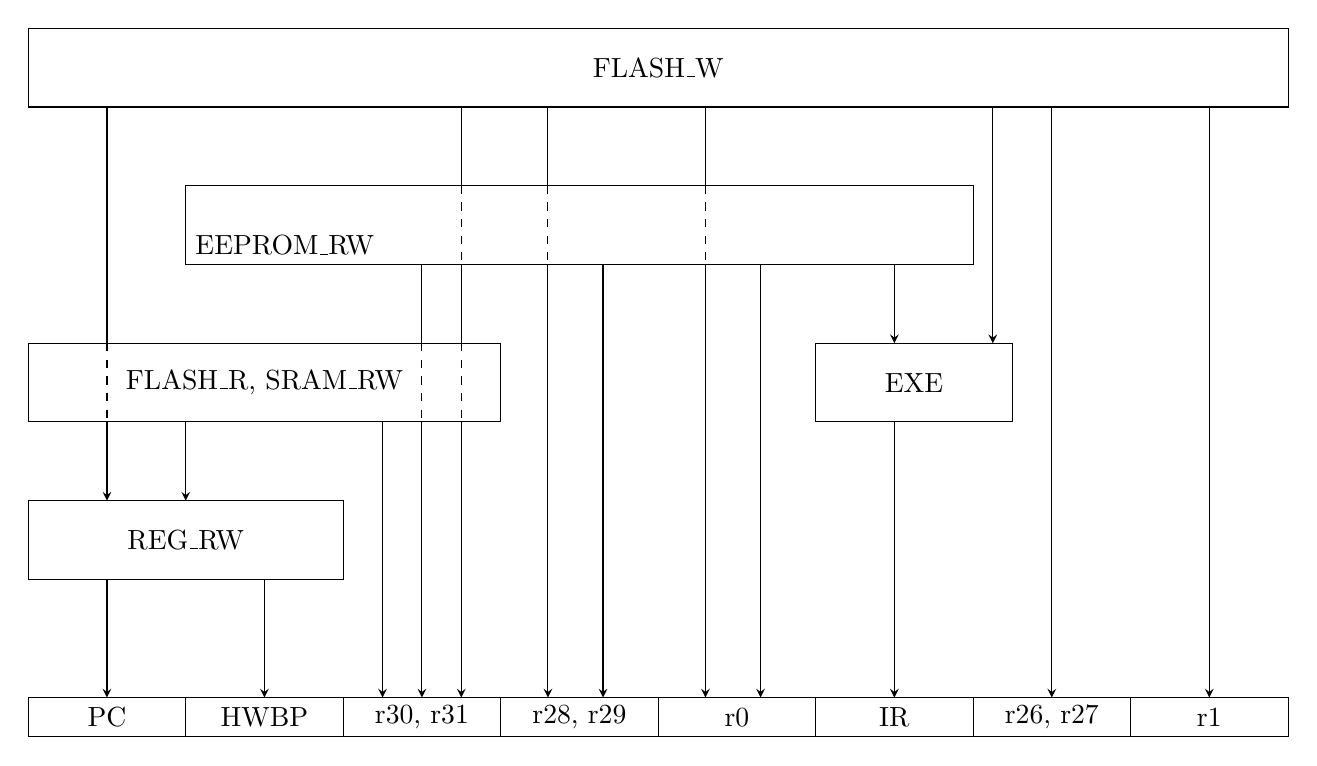
\begin{tikzpicture}
            \draw (0,0) rectangle (2, 0.5) node[pos=.5] {PC};
            \draw (2,0) rectangle (4, 0.5) node[pos=.5] {HWBP};
            \draw (4,0) rectangle (6, 0.5) node[pos=.5] {r30, r31};
            \draw (6,0) rectangle (8, 0.5) node[pos=.5] {r28, r29};
            \draw (8,0) rectangle (10, 0.5) node[pos=.5] {r0};
            \draw (10,0) rectangle (12, 0.5) node[pos=.5] {IR};
            \draw (12,0) rectangle (14, 0.5) node[pos=.5] {r26, r27};
            \draw (14,0) rectangle (16, 0.5) node[pos=.5] {r1};
            \draw (0, 2) rectangle (4, 3) node[pos=.5] {REG\_RW};
            \draw (0, 4) rectangle (6, 5) node[pos=.5] {FLASH\_R, SRAM\_RW};
            \draw (10, 4) rectangle (12.5, 5) node[pos=.5] {EXE};
            \draw (12, 7) rectangle (2, 6) node[anchor=south west] {EEPROM\_RW};
            \draw (0, 8) rectangle (16, 9) node[pos=.5] {FLASH\_W};

            \draw [-stealth](1, 2) -- (1, 0.5);
            \draw [-stealth](3, 2) -- (3, 0.5);
            \draw [-stealth](4.5, 4) -- (4.5, 0.5);
            \draw [-stealth](7.3, 6) -- (7.3, 0.5);
            \draw [-stealth](9.3, 6) -- (9.3, 0.5);
            \draw [-stealth](11, 4) -- (11, 0.5);
            \draw [-stealth](13, 8) -- (13, 0.5);
            \draw [-stealth](15, 8) -- (15, 0.5);

            \draw [-stealth](2, 4) -- (2, 3);
            \draw [-stealth](11, 6) -- (11, 5);
            \draw [-stealth](12.25, 8) -- (12.25, 5);

            \draw (6.6, 8) -- (6.6, 7);
            \draw [dashed](6.6, 7) -- (6.6, 6);
            \draw [-stealth](6.6, 6) -- (6.6, 0.5);

            \draw (8.6, 8) -- (8.6, 7);
            \draw [dashed](8.6, 7) -- (8.6, 6);
            \draw [-stealth](8.6, 6) -- (8.6, 0.5);

            \draw (1, 8) -- (1, 5);
            \draw [dashed](1, 5) -- (1, 4);
            \draw [-stealth](1, 4) -- (1, 3);

            \draw (5, 6) -- (5, 5);
            \draw [dashed](5, 5) -- (5, 4);
            \draw [-stealth](5, 4) -- (5, 0.5);

            \draw (5.5, 8) -- (5.5, 7);
            \draw [dashed](5.5, 7) -- (5.5, 6);
            \draw (5.5, 6) -- (5.5, 5);
            \draw [dashed](5.5, 5) -- (5.5, 4);
            \draw [-stealth](5.5, 4) -- (5.5, 0.5);
        \end{tikzpicture}
    }

    \caption[]{Diagramma delle dipendenze di utilizzo dei registri target per le azioni DebugWire}\label{fig:dw-wrt-deps}
\end{figure}

È possibile individuare un cammino comune di salvataggio e ripristino dei registri per tutte le operazioni. In particolare è evidente come tutte le operazioni, ad eccezione di \texttt{EXE}, dipendano da \texttt{REG\_RW}, e come le operazioni di scrittura sulle memorie non volatili dipendano da scritture sugli stessi registri di \texttt{SRAM\_RW}.

La sequenza di salvataggio e ripristino viene mostrata nella la figura~\ref{fig:dw-wrt-seq}. L'immagine mostra una pila di registri per la quale, dato un punto di ingresso comune in funzione dell'azione da eseguire, sarà necessario salvare tutti i registri visitati nella discesa della pila fino al punto di uscita definito da tale operazione. Per esempio, l'azione \texttt{EEPROM\_RW} dovrà salvare i registri \texttt{PC}, \texttt{HWBP}, \texttt{Z (r30, r31)}, \texttt{IR}, \texttt{Y(r26, r27)} e \texttt{r0}. È possibile notare come i registri elencati siano anche quelli utilizzati dal codice presente al documento in appendice~\ref{app:dw-eeprom-prog}

\begin{figure}[h]
    \centering
    %\resizebox{.95\textwidth}{!}{%
        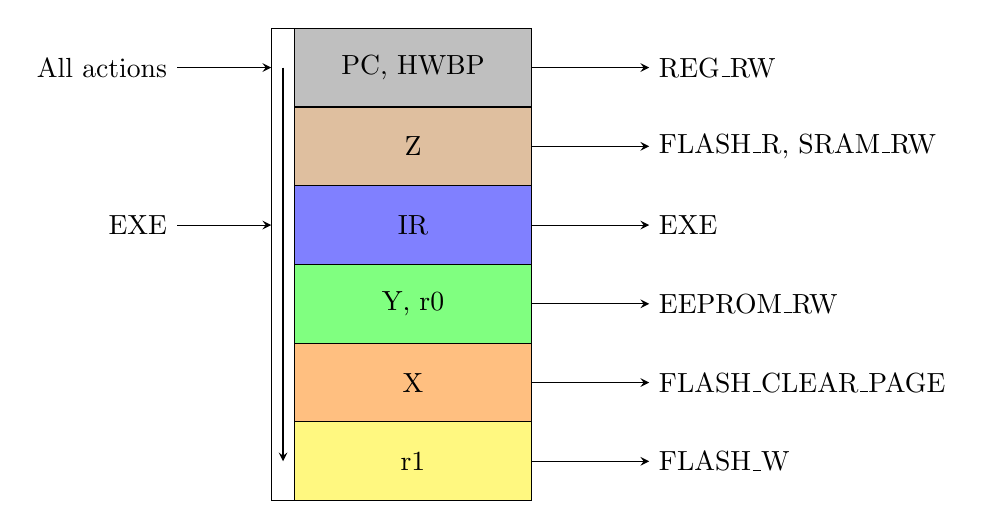
\begin{tikzpicture}
            
            \draw [fill=yellow!50] (0,0) rectangle (3, 1) node[pos=.5] {r1};
            \draw [fill=orange!50] (0,1) rectangle (3, 2) node[pos=.5] {X};
            \draw [fill=green!50] (0,2) rectangle (3, 3) node[pos=.5] {Y, r0};
            \draw [fill=blue!50] (0,3) rectangle (3, 4) node[pos=.5] {IR};
            \draw [fill=brown!50] (0,4) rectangle (3, 5) node[pos=.5] {Z};
            \draw [fill=gray!50] (0,5) rectangle (3, 6) node[pos=.5] {PC, HWBP};

            \draw (-0.3, 0) rectangle (0, 6);
            \draw [-stealth] (-0.15, 5.5) -- (-0.15, 0.5);

            \draw [stealth-] (-0.3, 5.5) -- (-1.5, 5.5) node[left] {All actions};
            \draw [stealth-] (-0.3, 3.5) -- (-1.5, 3.5) node[left] {EXE};

            \draw [-stealth] (3, 5.5) -- (4.5, 5.5) node[right] {REG\_RW};
            \draw [-stealth] (3, 4.5) -- (4.5, 4.5) node[right] {FLASH\_R, SRAM\_RW};
            \draw [-stealth] (3, 2.5) -- (4.5, 2.5) node[right] {EEPROM\_RW};
            \draw [-stealth] (3, 1.5) -- (4.5, 1.5) node[right] {FLASH\_CLEAR\_PAGE};
            \draw [-stealth] (3, 0.5) -- (4.5, 0.5) node[right] {FLASH\_W};
            \draw [-stealth] (3, 3.5) -- (4.5, 3.5) node[right] {EXE};
        \end{tikzpicture}
    %}

    \caption[]{Diagramma dei salvataggi e ripristini dei registri in funzione dell'operazione da eseguire}\label{fig:dw-wrt-seq}
\end{figure}

\subsection{Software Breakpoints}

L'aggiunta della possibilità di scrivere la memoria flash consente l'implementazione dei software breakpoints.

Un breakpoint è un indicatore associato a un indirizzo di memoria dove il codice è in esecuzione con il fine di interrompere l'esecuzione dell'algoritmo e passare il controllo al debugger per effettuare le operazioni di analisi e ispezione.

Questi consistono nella sovrascrittura di un'istruzione con l'opcode corrispondente a \texttt{BREAK} causando così l'halt della cpu e l'intervento del debugger prima dell'esecuzione della stessa.
Alla ripresa dell'esecuzione il debugger caricherà in memoria l'istruzione originale e riprenderà il flusso del codice.

Un primo approccio per la scrittura del codice relativo a questa feature consiste nell'aggiornare la memoria flash scrivendo un'istruzione BREAK\footnote{0x0000} non appena possibile e salvare in una struttura dati la coppia \[<indirizzo>:<opcode>\]

Un possibile algoritmo viene esibito di seguito. Questo algoritmo ha un impatto sull'utilizzo della memoria SRAM di 18 byte facendo uso del fatto che è possibile riempire il buffer di scrittura prima della cancellazione della pagina.

Sia \(address\) l'indirizzo dell'istruzione da sostituire (word address), \(pagelen\) il numero di word in una pagina.

\begin{enumerate}
    \item Salvataggio dei registri come definito in figura~\ref{fig:dw-wrt-seq} per l'azione \texttt{FLASH\_W} (14 byte)
    \item Poniamo l'indirizzo di pagina, utilizzando 2 byte, come \[pageaddr = \left\lfloor\frac{address}{pagelen}\right\rfloor pagelen\] 
    \item Iniziamo la scrittura di una pagina e, per ogni indirizzo da \(pageaddr\) a \(address\) (escluso), leggiamo in una variabile temporanea (2 byte) il valore della memoria flash a quell'indirizzo e aggiungiamo al buffer di scrittura presente nell'integrato.
    \item Scriviamo del buffer l'istruzione BREAK.\@ 
    \item Per ogni indirizzo da \(address + 1\) a \(pageaddr + pagelen - 1\) popoliamo il buffer con quanto letto. 
    \item Eseguiamo l'azione Page Clear all'indirizzo \(pageaddr\)
    \item Eseguiamo l'azione di programmazione della pagina.
    \item Ripristiniamo lo stato dei registri invertendo quanto eseguito al punto 1.
\end{enumerate}

Quanto riportato, seppur una soluzione valida, causa un deterioramento della memoria flash e innalza notevolmente i tempi di debug, inserendo attese notevoli tra il posizionamento di un breakpoint e un altro.

L'algoritmo finale risolve queste problematiche adottando una gestione ``\textit{lazy}'' dei breakpoint e accorpando modifiche alle pagine di memoria flash solo al momento precedente all'esecuzione.
Questo permette di evitare tutte le riscritture date dall'eventuale indecisione del programmatore o errori di puntamento.

Un breakpoint software viene definito con la struttura presentata nel listato~\ref{lst:dw-swbp-struct}. I flag \texttt{active} e \texttt{stored} permettono di identificare le azioni da intraprendere al momento dell'applicazione delle modifiche in memoria.

\noindent\begin{minipage}{\textwidth}
    \begin{lstlisting}[style=C, caption={Struttura utilizzata per il salvataggio dei riferimenti ai breakpoint software}, label=lst:dw-swbp-struct]
    typedef struct dw_sw_brkpt{
        uint16_t address;
        uint16_t opcode;

        uint8_t active : 1;
        uint8_t stored : 1;
    } dw_sw_brkpt_t;
    \end{lstlisting}
\end{minipage}

In particolare si ha che è necessario eseguire un'azione in memoria se i due flag sono discordanti: se un breakpoint è stato abilitato ma non è stato scritto in memoria sarà necessario sostituire l'istruzione presente all'indirizzo \(address\), mentre se un breakpoint è salvato (\texttt{stored} = 1) ma disabilitato sarà necessario ripristinare \(opcode\) all'indirizzo specificato.

Nel caso di aggiunta o rimozione di un breakpoint l'indirizzo viene ricercato all'interno della lista di breakpoint precedentemente definiti comparando l'indirizzo. Se il breakpoint era stato precedentemente definito allora il riferimento viene modificato impostando la variabile \texttt{active} al valore consono. In caso contrario viene creato un nuovo riferimento in coda.

Prima della ripresa dell'esecuzione la lista di breakpoint viene ordinata mediante insertion sort secondo in seguenti criteri:
\begin{itemize}
    \item se due riferimenti sono entrambi non salvati e inattivi non viene effettuata l'inversione e sono considerati uguali ignorando l'indirizzo.
    \item se il primo riferimento è inattivo e non salvato mentre il secondo è o salvato o attivato, allora viene eseguita l'inversione
    \item se sono tutti e due attivi o salvati, vengono comparati gli indirizzi e avviene l'inversione se il primo indirizzo è maggiore del secondo.
\end{itemize}

Così facendo si ottiene una lista di riferimenti ordinati per indirizzo crescente con i riferimenti da eliminare posti in coda a scapito di quest'ultimo, permettendo quindi la rimozione dei riferimenti inattivi e non salvati perché non più esistenti partendo dal fondo e eliminando fino a trovare un riferimento attivo o salvato.

Ora risulta possibile accorpare le scritture in memoria con un algoritmo simile a quanto riportato in precedenza considerando però la presenza di più breakpoint per pagina.

Sarebbe possibile rendere la ricerca e l'ordinamento più efficiente utilizzando algoritmi quali ricerca binaria e qsort ma non è stati ritenuto necessario essendo il numero massimo di riferimenti limitato a 20.

\section{Modifiche hardware alla scheda}\label{s:dw-board-mod}

Come discusso nell'introduzione la scheda \textit{Arduino UNO R3} non presenta alcun supporto al debugging o ad estensioni per tale funzione.

Questo comporta la necessità di sviluppare una nuova scheda derivata dall'architettura di \textit{Arduino UNO} --- il cui sviluppo comporterebbe un dispendio di energie e tempo non indifferenti e alte possibilità di errore --- oppure la modifica hardware e firmware di un esemplare della stessa.

Affinché sia possibile utilizzare l'interfaccia di debugging DebugWire è necessaria una connessione con pull-up diretta con il pin i reset dell'integrato.

Come è possibile osservare dall'allegato~\ref{app:r3-schematic}, L'integrato \texttt{U3} è connesso al pin di reset del target (\texttt{U4}) tramite il condensatore \texttt{C5} (si veda la figura~\ref{fig:r3-schematic-rst-detail}). Sarà dunque necessario rimuovere tale condensatore e ripristinare una connessione diretta tra i micro-controllori come evidenziato dalla figura~\ref{fig:remove-c5}.

\begin{figure}[t]
    \hfill
    \begin{minipage}{.45\textwidth}
        \subfloat[][]{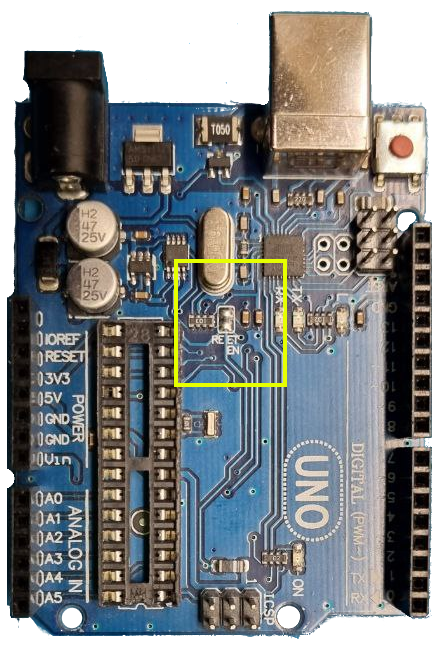
\includegraphics[width=.9\textwidth]{cap_begin.png}}
    \end{minipage}
    \begin{minipage}{.45\textwidth}
        \subfloat[][]{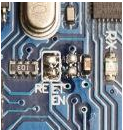
\includegraphics[width=.5\textwidth]{cap_removed.png}} \\
        \subfloat[][]{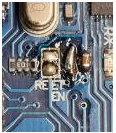
\includegraphics[width=.5\textwidth]{cap_shorted.png}}
    \end{minipage}
    \hfill
    \caption[]{Procedimento di rimozione del condensatore \texttt{C5}. Il condensatore viene rimosso (b) e successivamente la connessione viene ripristinata (c)}\label{fig:remove-c5}
\end{figure}

Tale modifica rende inoperabile il firmware presente sul controllore ATMega16U2 in quanto così facendo la linea di reset rimarrebbe asserita al livello logico 0 durante la durata della connessione con l'\texttt{host}.

Questa modifica comporta però il collegamento i componenti \texttt{RN2D} e \texttt{RN1D} i quali vanno a costituire un partitore di tensione che porrebbe la linea di reset ad un livello logico indefinito ad una tensione di 0.45V. Per questo motivo si rende necessaria una seconda modifica: è necessario isolare la resistenza \texttt{RN2D} tagliando la traccia come mostrato in figura~\ref{fig:cut-rnd2}

\begin{figure}[b]
    \centering
    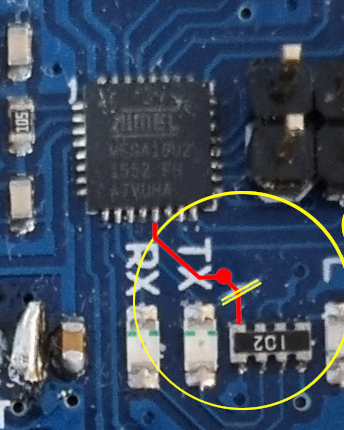
\includegraphics[width=.25\textwidth]{cut_rnd2.png}
    \caption[]{Isolamento del componente \texttt{RN2D} tagliando la traccia evidenziata.}\label{fig:cut-rnd2}
\end{figure}

Questa modifica si ripercuote negativamente sulla possibilità di eseguire il bootloader sull'ATMega16U2, in quanto è necessario che il pin 13 sia posto a 0V perchè esso possa essere caricato. Vi sono quindi tre possibilità:
\begin{enumerate}
    \item Caricare il firmware personalizzato antecedentemente alle modifiche hardware.
    \item Utilizzare un programmatore esterno tramite l'header di programmazione \texttt{ICSP1}
    \item Collegare temporaneamente durante il reset dell'ATMega16U2 la traccia tagliata con l'ausilio di uno strumento conduttivo.
\end{enumerate} 

\subsection{Riutilizzo del pulsante di reset}

La connessione per il debugging, trattasi di una linea seriale open drain, comporta che il punsante di reset presente sulla scheda non sia più funzionante, in quanto le funzionalità originali del pin di reset vengono disattivate con l'attivazione della periferica DebugWire.

La soluzione adottata consiste nell'implementazione di un soft-reset gestito dal microcontrollore ATMega16U2: La connessione del pulsante viene modificata in modo che esso sia un input letto dal firmware modificato del micro-controllore adattatore, il quale si occuperà di resettare il \textit{target} mediante l'invio di una sequenza di comandi descritta dall'algoritmo seguente:
\begin{enumerate}
    \item Halt del target (BREAK)
    \item Reset del controllore (0x07)
    \item Ripresa dell'esecuzione (0x30)
\end{enumerate}

A tal fine è necessario installare una connessione ausiliaria tramite un filo e tagliare la traccia di connessione del pulsante come mostrato dalla figura~\ref{fig:rst-rewire}

\begin{figure}[h]
    \centering
    \subfloat[][]{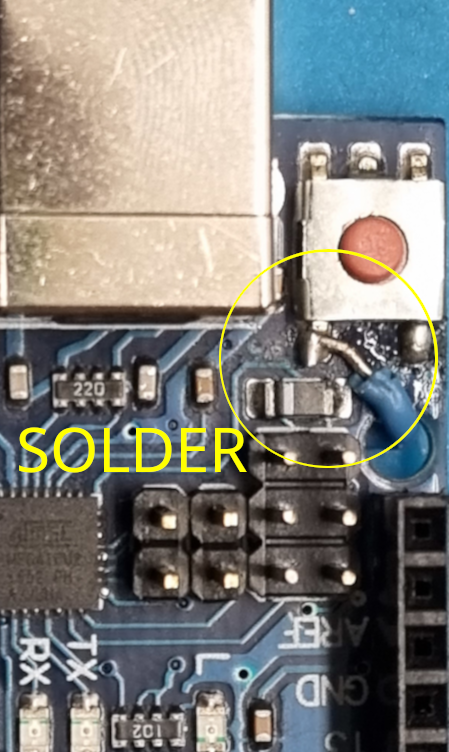
\includegraphics[width=.2\textwidth]{rst-solder-front.png}}
    \hspace{8mm}
    \subfloat[][]{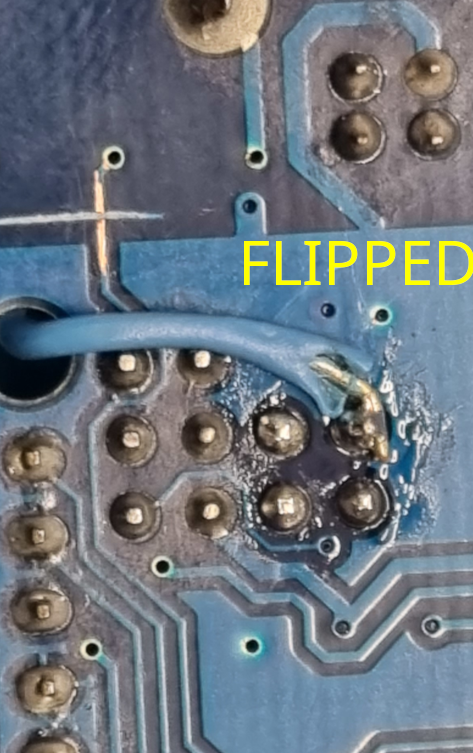
\includegraphics[width=.2\textwidth]{rst-solder-rear.png}}

    \caption[]{Procedimento di isolamento e riutilizzo del pulsante di reset mostrato dal lato superiore (a) e inferiore (b). Si noti la traccia tagliata nell'immagine (b)}\label{fig:rst-rewire}
\end{figure}

